\documentclass[ignorenonframetext,]{beamer}
\setbeamertemplate{caption}[numbered]
\setbeamertemplate{caption label separator}{: }
\setbeamercolor{caption name}{fg=normal text.fg}
\usepackage{lmodern}
\usepackage{amssymb,amsmath}
\usepackage{ifxetex,ifluatex}
\usepackage{fixltx2e} % provides \textsubscript
\ifnum 0\ifxetex 1\fi\ifluatex 1\fi=0 % if pdftex
  \usepackage[T1]{fontenc}
  \usepackage[utf8]{inputenc}
\else % if luatex or xelatex
  \ifxetex
    \usepackage{mathspec}
  \else
    \usepackage{fontspec}
  \fi
  \defaultfontfeatures{Ligatures=TeX,Scale=MatchLowercase}
  \newcommand{\euro}{€}
\fi
% use upquote if available, for straight quotes in verbatim environments
\IfFileExists{upquote.sty}{\usepackage{upquote}}{}
% use microtype if available
\IfFileExists{microtype.sty}{%
\usepackage{microtype}
\UseMicrotypeSet[protrusion]{basicmath} % disable protrusion for tt fonts
}{}
\newif\ifbibliography
\usepackage{color}
\usepackage{fancyvrb}
\newcommand{\VerbBar}{|}
\newcommand{\VERB}{\Verb[commandchars=\\\{\}]}
\DefineVerbatimEnvironment{Highlighting}{Verbatim}{commandchars=\\\{\}}
% Add ',fontsize=\small' for more characters per line
\usepackage{framed}
\definecolor{shadecolor}{RGB}{248,248,248}
\newenvironment{Shaded}{\begin{snugshade}}{\end{snugshade}}
\newcommand{\KeywordTok}[1]{\textcolor[rgb]{0.13,0.29,0.53}{\textbf{{#1}}}}
\newcommand{\DataTypeTok}[1]{\textcolor[rgb]{0.13,0.29,0.53}{{#1}}}
\newcommand{\DecValTok}[1]{\textcolor[rgb]{0.00,0.00,0.81}{{#1}}}
\newcommand{\BaseNTok}[1]{\textcolor[rgb]{0.00,0.00,0.81}{{#1}}}
\newcommand{\FloatTok}[1]{\textcolor[rgb]{0.00,0.00,0.81}{{#1}}}
\newcommand{\ConstantTok}[1]{\textcolor[rgb]{0.00,0.00,0.00}{{#1}}}
\newcommand{\CharTok}[1]{\textcolor[rgb]{0.31,0.60,0.02}{{#1}}}
\newcommand{\SpecialCharTok}[1]{\textcolor[rgb]{0.00,0.00,0.00}{{#1}}}
\newcommand{\StringTok}[1]{\textcolor[rgb]{0.31,0.60,0.02}{{#1}}}
\newcommand{\VerbatimStringTok}[1]{\textcolor[rgb]{0.31,0.60,0.02}{{#1}}}
\newcommand{\SpecialStringTok}[1]{\textcolor[rgb]{0.31,0.60,0.02}{{#1}}}
\newcommand{\ImportTok}[1]{{#1}}
\newcommand{\CommentTok}[1]{\textcolor[rgb]{0.56,0.35,0.01}{\textit{{#1}}}}
\newcommand{\DocumentationTok}[1]{\textcolor[rgb]{0.56,0.35,0.01}{\textbf{\textit{{#1}}}}}
\newcommand{\AnnotationTok}[1]{\textcolor[rgb]{0.56,0.35,0.01}{\textbf{\textit{{#1}}}}}
\newcommand{\CommentVarTok}[1]{\textcolor[rgb]{0.56,0.35,0.01}{\textbf{\textit{{#1}}}}}
\newcommand{\OtherTok}[1]{\textcolor[rgb]{0.56,0.35,0.01}{{#1}}}
\newcommand{\FunctionTok}[1]{\textcolor[rgb]{0.00,0.00,0.00}{{#1}}}
\newcommand{\VariableTok}[1]{\textcolor[rgb]{0.00,0.00,0.00}{{#1}}}
\newcommand{\ControlFlowTok}[1]{\textcolor[rgb]{0.13,0.29,0.53}{\textbf{{#1}}}}
\newcommand{\OperatorTok}[1]{\textcolor[rgb]{0.81,0.36,0.00}{\textbf{{#1}}}}
\newcommand{\BuiltInTok}[1]{{#1}}
\newcommand{\ExtensionTok}[1]{{#1}}
\newcommand{\PreprocessorTok}[1]{\textcolor[rgb]{0.56,0.35,0.01}{\textit{{#1}}}}
\newcommand{\AttributeTok}[1]{\textcolor[rgb]{0.77,0.63,0.00}{{#1}}}
\newcommand{\RegionMarkerTok}[1]{{#1}}
\newcommand{\InformationTok}[1]{\textcolor[rgb]{0.56,0.35,0.01}{\textbf{\textit{{#1}}}}}
\newcommand{\WarningTok}[1]{\textcolor[rgb]{0.56,0.35,0.01}{\textbf{\textit{{#1}}}}}
\newcommand{\AlertTok}[1]{\textcolor[rgb]{0.94,0.16,0.16}{{#1}}}
\newcommand{\ErrorTok}[1]{\textcolor[rgb]{0.64,0.00,0.00}{\textbf{{#1}}}}
\newcommand{\NormalTok}[1]{{#1}}

% Prevent slide breaks in the middle of a paragraph:
\widowpenalties 1 10000
\raggedbottom

% Comment these out if you don't want a slide with just the
% part/section/subsection/subsubsection title:
\AtBeginPart{
  \let\insertpartnumber\relax
  \let\partname\relax
  \frame{\partpage}
}
\AtBeginSection{
  \ifbibliography
  \else
    \let\insertsectionnumber\relax
    \let\sectionname\relax
    \frame{\sectionpage}
  \fi
}
\AtBeginSubsection{
  \let\insertsubsectionnumber\relax
  \let\subsectionname\relax
  \frame{\subsectionpage}
}

\setlength{\emergencystretch}{3em}  % prevent overfull lines
\providecommand{\tightlist}{%
  \setlength{\itemsep}{0pt}\setlength{\parskip}{0pt}}
\setcounter{secnumdepth}{0}

\title{MCMC Tutorial}
\subtitle{A short introduction to Bayesian Analysis and Metropolis-Hastings MCMC}
\author{Ralph Schlosser}
\date{February 2017}
% Some style additions.
% RS09022015

% Set the logo.
\pgfdeclareimage[height=0.8cm, width=0.8cm]{logo}{logo.png}
%\logo{\pgfuseimage{logo}\vspace{260pt}}
\logo{\pgfuseimage{logo}}

% Some style settings.
\usetheme{Madrid}
%\usefonttheme{serif}
\usecolortheme{beaver}

% Set additional fields.
\institute[]{\href{https://github.com/bwv988}{https://github.com/bwv988}}

% Further beamer settings.
\setbeamertemplate{navigation symbols}{}
% Some style additions.
% RS09022015

\usepackage{color}
\usepackage{graphicx}
\usepackage{subcaption}
\usepackage{mathtools}
\usepackage{grffile}
\newcommand{\mat}[1]{\mathbf{#1}}
\newcommand{\expt}[1]{\mathbb{E}({#1})}
\newcommand{\hvec}[1]{\hat{\underline{#1}}}
\renewcommand{\vec}[1]{\underline{#1}}

\newcommand{\FIXME}[1]{\noindent{\color{red} FIXME: #1}
}

\newcommand{\HIGHLIGHT}[1]{\noindent{\color{blue}#1}}

\newcommand{\orange}[1]{\textcolor{orange}{#1}}


\DeclarePairedDelimiter\floor{\lfloor}{\rfloor}

\begin{document}
\frame{\titlepage}

\begin{frame}{Overview}

\begin{itemize}
\tightlist
\item
  Bayesian Analysis
\item
  Monte Carlo Integration
\item
  Sampling Methods
\item
  Markov Chain Monte Carlo
\item
  Metropolis-Hastings Algorithm
\item
  Example: Linear Regression and M-H MCMC
\item
  Outlook
\end{itemize}

\end{frame}

\begin{frame}{Bayesian Analysis: Introduction}

\begin{columns}
  \column{0.6\textwidth}
  \begin{itemize}
    \item Foundation for MCMC: \HIGHLIGHT{Bayesian Analysis}.
    \item \HIGHLIGHT{Frequentist} -- Likelihood model: $p(\vec{x} | \vec{\theta})$
    \item How likely are the data $\vec{x}$, given the fixed parameters $\vec{\theta}$.
    \item In general we want to estimate $\vec{\theta}$, e.g. through MLE.
    \item \HIGHLIGHT{Bayesian} -- Bayesian model: $p(\vec{\theta} | \vec{x})$.
    \item Fundamental difference: In Bayesian analysis, both parameter model \orange{and} data are treated as random variables.
  \end{itemize}
  \column{0.4\textwidth}
  \begin{figure}
    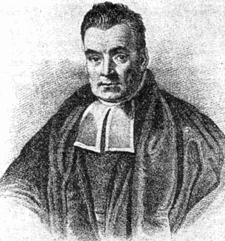
\includegraphics[scale=0.5]{images/bayes.png}
    \caption*{\tiny Thomas Bayes (1707-1761)}
  \end{figure}
\end{columns}

\end{frame}

\begin{frame}{Bayesian Analysis: Terminology}

\begin{itemize}
\tightlist
\item
  From \HIGHLIGHT{joint probability} distribution to
  \HIGHLIGHT{posterior distribution} via data \HIGHLIGHT{likelihood} and
  \HIGHLIGHT{prior beliefs}:
\end{itemize}

\[
\begin{aligned}
p(x, \theta) &= p(x | \theta) p(\theta)\\
p(\theta | x) &= \frac{p(x, \theta)}{p(x)}\\
&= \frac{p(x | \theta) p(\theta)}{p(x)} 
\end{aligned}
\]

\begin{itemize}
\tightlist
\item
  Normalizing term \(p(x)\) difficult to get, but often not needed:
\end{itemize}

\[
\begin{aligned}
p(\theta | x) & \propto p(x | \theta) p(\theta)
\end{aligned}
\]

\begin{itemize}
\tightlist
\item
  \orange{Posterior $\propto$ likelihood $\times$ prior}
\end{itemize}

\end{frame}

\begin{frame}{Bayesian Analysis: Pros and Cons}

\begin{itemize}
\item
  \HIGHLIGHT{Pro}: Common-sense interpretability of results, e.g.
  \emph{Credible Intervals} vs.~classical Confidence Intervals.
\item
  \HIGHLIGHT{Pro}: Update model parameters as new data becomes
  available.
\item
  \HIGHLIGHT{Pro}: Create \emph{hierarchical models} through chaining:

  \begin{itemize}
  \tightlist
  \item
    \(p(\phi, \theta | x) = p(x |\phi, \theta) p(\theta | \phi) p(\phi)\)
  \item
    Hyperprior: \(p(\theta | \phi) p(\phi)\)
  \item
    \emph{Yesterdays posterior is tomorrow's prior}
  \end{itemize}
\item
  \orange{Con}: \textbf{Must} have a joint model for parameters, data,
  and prior.

  \begin{itemize}
  \tightlist
  \item
    What if we have absolutely no prior information?
  \end{itemize}
\item
  \orange{Con}: Choice of prior considered to be subjective.
\item
  \orange{Con}: Subjectiveness makes comparison difficult.
\end{itemize}

\end{frame}

\begin{frame}{Bayesian Analysis: Applications}

\begin{itemize}
\tightlist
\item
  Inferences and predictions in a Bayesian setting:
\end{itemize}

\[
\begin{aligned}
p(\theta | x) &= \frac{p(x | \theta) p(\theta)}{\int_{\Theta} p(x | \theta') p(\theta')  d \theta'} & \mbox{Normalization}\\
p(\tilde{y} | y) &= \int_{\Theta} p(\tilde{y} | \theta') p(\theta' | y)  d \theta' & \mbox{Predict new data}
\end{aligned}
\]

\begin{itemize}
\tightlist
\item
  Posterior summary statistics, e.g.~expectations:
\end{itemize}

\[
\begin{aligned}
\mathbb{E}_{p}(g(\theta) | x) &= \int_{\Theta} g(\theta') p(\theta' | x) d\theta'\\
\mbox{mean: } g(\theta) = \theta
\end{aligned}
\]

\begin{itemize}
\tightlist
\item
  Many classical models can be expressed in a Bayesian context, like
  e.g.~linear regression, ARMA, GLMs, etc.
\item
  \HIGHLIGHT{Missing data}: Natural extension.
\end{itemize}

\end{frame}

\begin{frame}{Monte Carlo Integration: Introduction}

\begin{itemize}
\tightlist
\item
  Applied Bayesian analysis asks to \orange{integrate} over (often
  analytically intractable) posterior densities.
\item
  \HIGHLIGHT{Solution}: \textbf{Monte Carlo Integration}
\item
  Suppose we wish to evaluate
  \(\mathbb{E}_{p}(g(\theta) | x) = \int_{\Theta} g(\theta') p(\theta' | x) d\theta'\)
\item
  Given a set of \(N\) \orange{i.i.d. samples}
  \(\theta_1, \theta_2, ..., \theta_N\) from the density \(p\):
\end{itemize}

\[
\begin{aligned}
\mathbb{E}_{p}(g(\theta | x)) & \approx \frac{1}{N} \sum_{i = 1}^{N} g(\theta_i)
\end{aligned}
\]

\begin{itemize}
\tightlist
\item
  \HIGHLIGHT{But}: Need to be able to draw random samples from \(p\)!
\end{itemize}

\end{frame}

\begin{frame}[fragile]{Monte Carlo Integration: Example}

Simulate \(N=10000\) draws from a univariate standard normal, i.e.
\(X \sim N(0, 1)\). Let \(p(x)\) be the normal density. Then:

\[
\begin{aligned}
P(X \le 0.5) &= \int_{-\infty}^{0.5} p(x) dx
\end{aligned}
\]

\begin{Shaded}
\begin{Highlighting}[]
\KeywordTok{set.seed}\NormalTok{(}\DecValTok{123}\NormalTok{)}
\NormalTok{data <-}\StringTok{ }\KeywordTok{rnorm}\NormalTok{(}\DataTypeTok{n =} \DecValTok{10000}\NormalTok{)}
\NormalTok{prob.in <-}\StringTok{ }\NormalTok{data <=}\StringTok{ }\FloatTok{0.5}
\KeywordTok{sum}\NormalTok{(prob.in) /}\StringTok{ }\DecValTok{10000}
\end{Highlighting}
\end{Shaded}

\begin{verbatim}
## [1] 0.694
\end{verbatim}

\begin{Shaded}
\begin{Highlighting}[]
\KeywordTok{pnorm}\NormalTok{(}\FloatTok{0.5}\NormalTok{)}
\end{Highlighting}
\end{Shaded}

\begin{verbatim}
## [1] 0.6914625
\end{verbatim}

\end{frame}

\begin{frame}{Sampling Methods}

\begin{itemize}
\tightlist
\item
  Sampling from the posterior distribution is really important.
\item
  Classical sampling methods:

  \begin{itemize}
  \tightlist
  \item
    Inversion sampling
  \item
    Importance sampling
  \item
    Rejection sampling
  \end{itemize}
\item
  Drawbacks:

  \begin{itemize}
  \tightlist
  \item
    Closed-form expression rarely accessible (Method of Inversion).
  \item
    Doesn't generalize well for \orange{highly-dimensional} problems.
  \end{itemize}
\item
  \HIGHLIGHT{Metropolis-Hastings MCMC} has largely superseded the above.
\end{itemize}

\end{frame}

\begin{frame}{Markov Chain Monte Carlo (MCMC)}

\begin{itemize}
\tightlist
\item
  Unlike pure Monte Carlo, in MCMC we create \HIGHLIGHT{dependent}
  samples.
\item
  Consider the \textbf{target distribution} \(p(\theta | x)\) which is
  only known up to proportionality.
\item
  Construct a Markov Chain in the state space of \(\theta \in \Theta\)
  with \orange{stationary distribution} \(p(\theta | x)\).
\item
  Markov property -- New state of chain depends only on previous state
  (\(K\): transitional kernel d.f.).
\end{itemize}

\[
\begin{aligned}
\theta_{t + 1} &= K(\theta | \theta_t) \\
\end{aligned}
\]

\begin{itemize}
\tightlist
\item
  With realizations \(\{\theta_t: t=0, 1, ...\}\) from the chain:
\end{itemize}

\[
\begin{aligned}
\theta_t & \rightarrow p(\theta | x) \\
\frac{1}{N} \sum_{t = 1}^{N} g(\theta_t) & \rightarrow \mathbb{E}_{p}(g(\theta | x)) \mbox{ a.s.}
\end{aligned}
\]

\end{frame}

\begin{frame}{Metropolis-Hastings MCMC: Intro \& some history}

\begin{itemize}
\tightlist
\item
  An implementation of MCMC.
\item
  Originally developed by researchers
  \HIGHLIGHT{Nicholas Metropolis, Stanislaw Ulam}, and co. at Los Alamos
  National Laboratories in the 1950's.
\item
  Generalized through work done by \orange{Hastings} in the 1970's.
\item
  Popularized by a 1990 research paper from
  \HIGHLIGHT{Gelfand \& Smith}:
  \url{http://wwwf.imperial.ac.uk/~das01/MyWeb/SCBI/Papers/GelfandSmith.pdf}
\item
  M-H MCMC really helped turning Bayesian analysis into practically
  useful tool.
\end{itemize}

\end{frame}

\begin{frame}{Metropolis-Hastings MCMC: Terminology}

\begin{itemize}
\tightlist
\item
  M-H has two main ingredients.
\item
  A \HIGHLIGHT{proposal distribution}.

  \begin{itemize}
  \tightlist
  \item
    Dependent on the current chain state \(\theta_t\), generate a
    candidate for the new state \(\phi\).
  \item
    Written as \(q(\theta_t, \phi)\).
  \item
    Can be chosen arbitrarily, but there are caveats (efficiency).
  \end{itemize}
\item
  An \orange{acceptance probability}.

  \begin{itemize}
  \tightlist
  \item
    Accept with probability \(\alpha\) the move from the current state
    \(\theta_t\) to state \(\phi\).
  \item
    Written as \(\alpha(\theta_t, \phi)\).
  \end{itemize}
\item
  Main idea behind M-H: With every step, we want to get closer to the
  target density (e.g.~posterior density).
\end{itemize}

\end{frame}

\begin{frame}{Metropolis-Hastings MCMC: Intuition}

\begin{itemize}
\tightlist
\item
  Let's call our \orange{target distribution} (from which we want to
  sample) \(\pi\).
\item
  At the core of the M-H algorithm we have the calculation of
  \(\alpha(\theta_t, \phi)\):
\end{itemize}

\[
\begin{aligned}
\alpha(\theta_t, \phi) = min \Big( 1, \frac{\pi(\phi) q(\phi, \theta_t)}{\pi(\theta_t) q(\theta_t, \phi)} \Big)
\end{aligned}
\]

\begin{itemize}
\tightlist
\item
  Often \(q\) is symmetric, in which case it cancels out.
\item
  If \(\frac{\pi(\phi)}{\pi({\theta_t})} > 1\) \(\rightarrow\) target
  density at the proposed \textbf{new} value is higher than at current
  value.
\item
  In this case, we will \HIGHLIGHT{accept} the move from \(\theta_t\) to
  \(\phi\) with probability 1.

  \begin{itemize}
  \tightlist
  \item
    \emph{M-H really loves upward moves} :)
  \end{itemize}
\item
  \textbf{Main point}: Working with ratios of \(\pi\), so only need
  \(\pi\) up to proportionality!
\end{itemize}

\end{frame}

\begin{frame}{Metropolis-Hastings MCMC: Algorithm}

\begin{enumerate}
\def\labelenumi{\arabic{enumi}.}
\tightlist
\item
  Initialize \(\theta_0\), number of iterations.
\item
  Given the current state \(\theta_t\), generate new state \(\phi\) from
  the proposal distribution \(q(\theta_t, \phi)\).
\item
  Calculate acceptance probability \(\alpha(\theta_t, \phi)\).
\item
  With probability \(\alpha(\theta_t, \phi)\), set
  \(\theta_{t + 1} = \phi\), else set \(\theta_{t + 1} = \theta_t\).
\item
  Iterate
\item
  Result: \HIGHLIGHT{Realizations} of dependent samples
  \(\{\theta_1, \theta_2, ...\}\) from the target distribution
  \(\pi(\theta)\).
\end{enumerate}

Using these dependent realizations \& due to the Monte Carlo approach,
we can now look at making inferences and predictions.

\end{frame}

\begin{frame}{Example: Linear Regression and M-H MCMC}

\begin{itemize}
\tightlist
\item
  Consider a simple linear model: \(y = \beta_1 x + \epsilon\).
\item
  As usual \(\epsilon \sim N(0, \sigma^2)\) with \(\sigma^2\) known.
\item
  We wish to make inferences on, e.g. \(\beta_1\).
\item
  Bayesian approach:
\end{itemize}

\[
\begin{aligned}
p(\beta_1 | y, x, \sigma^2) & = p(y | \beta_1, x, \sigma^2) p(\beta_1)
\end{aligned}
\]

\begin{itemize}
\tightlist
\item
  Let's choose a uniform prior for \(\beta_1\). We can now create
  samples using M-H MCMC.
\item
  See R code!
\end{itemize}

\end{frame}

\begin{frame}{Outlook}

\begin{itemize}
\tightlist
\item
  Many more interesting things could be mentioned, e.g.
  \orange{burn-in}, choice of \(q\), Gibbs-sampling etc.
\item
  M-H and Monte Carlo in deep learning:
  \url{http://www.deeplearningbook.org/contents/monte_carlo.html}
\item
  Bayesian Deep Learning is a \HIGHLIGHT{thing} (apparently, don't know
  anything about it!)
\item
  Went way over my head, but looks cool -- Finding the Higgs boson,
  featuring Monte Carlo \& Bayes:
  \url{http://hea-www.harvard.edu/AstroStat/Stat310_1314/dvd_20140121.pdf}
\item
  Along the same lines, the amazing NIPS 2016 keynote:
  \url{https://nips.cc/Conferences/2016/Schedule?showEvent=6195}
\item
  M-H in \orange{Latent Dirichlet Allocation}:
  \url{http://mlg.eng.cam.ac.uk/teaching/4f13/1112/lect10.pdf}
\end{itemize}

\end{frame}

\end{document}
